% Define block styles
\tikzstyle{block} = [draw, rectangle, text centered, text width=6cm, minimum height=1cm, rounded corners=true]
\tikzstyle{blockSmall} = [draw, rectangle, text centered, text width=2cm, minimum height=1cm, rounded corners=true]
\tikzstyle{arrowtext} = [text width=4em, text centered]
\tikzstyle{arrow} = [draw, -latex]

\definecolor{red1}{RGB}{160,0,0}
\definecolor{green1}{RGB}{0,160,0}
\definecolor{blue1}{RGB}{0,0,160}
	      
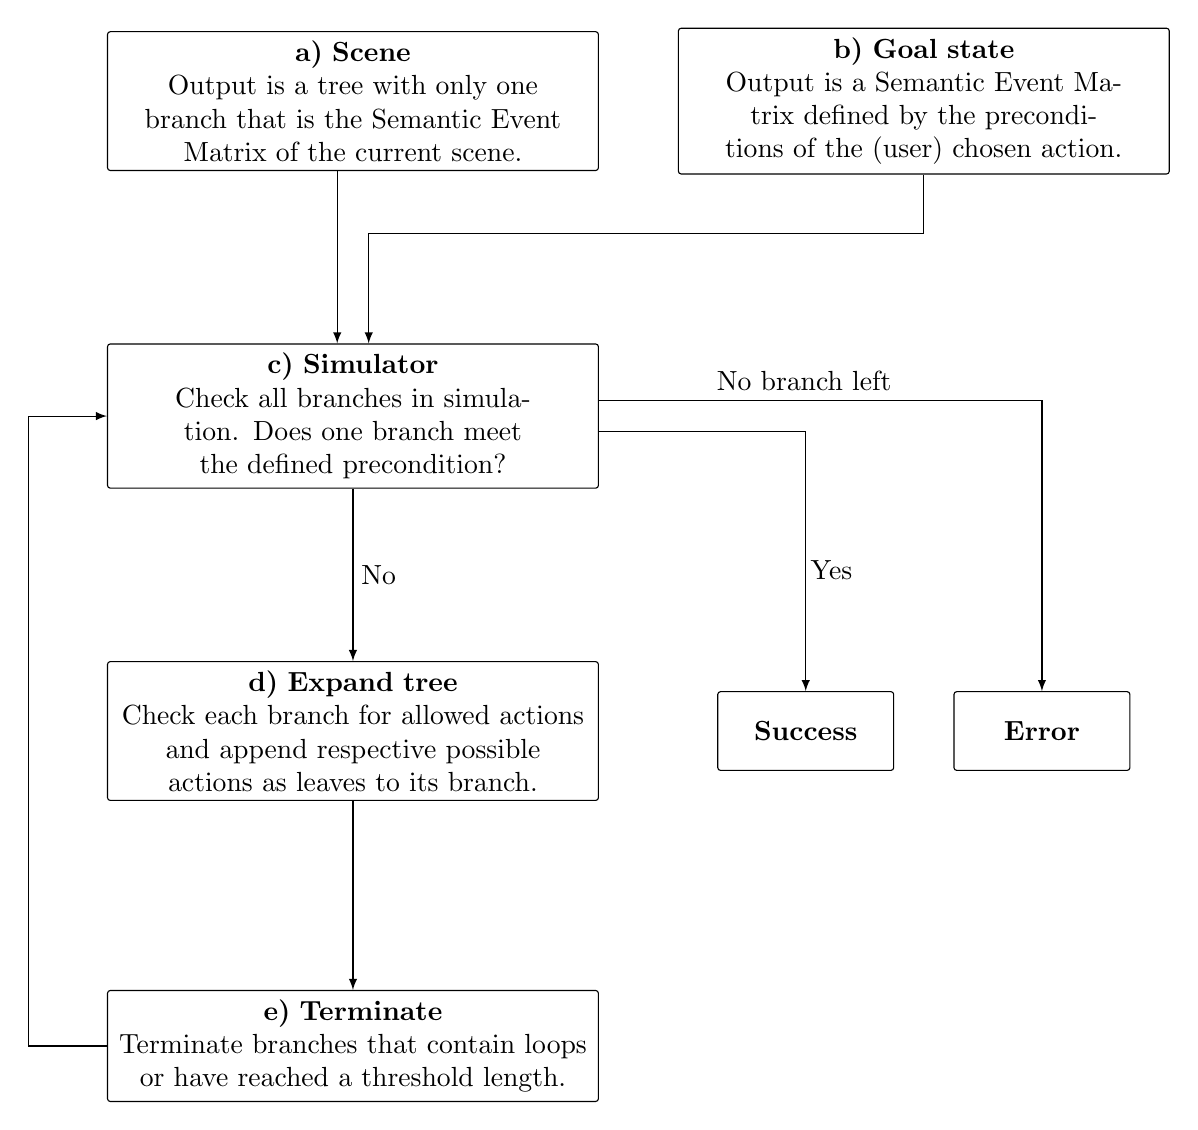
\begin{tikzpicture}[node distance=4.0cm, auto]
  \node [block] (scene) {\textbf{a) Scene}\\Output is a tree with only one branch that is the Semantic Event Matrix of the current scene.};
  \node [block, right of=scene, node distance=7.25cm] (goalstate) {\textbf{b) Goal state}\\Output is a Semantic Event Matrix defined by the preconditions of the (user) chosen action.};
  
  \node [block, below of=scene] (check) {\textbf{c) Simulator}\\Check all branches in simulation. Does one branch meet the defined precondition?};
  \node [block, below of=check] (tree) {\textbf{d) Expand tree}\\Check each branch for allowed actions and append respective possible actions as leaves to its branch.};
  \node [block, below of=tree] (terminate) {\textbf{e) Terminate}\\Terminate branches that contain loops or have reached a threshold length.};

  \node [blockSmall, below of=goalstate, xshift=-1.5cm, node distance=8cm] (success) {\textbf{Success}};
  \node [blockSmall, below of=goalstate, xshift= 1.5cm, node distance=8cm] (error) {\textbf{Error}};

  \draw [arrow] ([xshift=-0.2cm]scene.south) to ([xshift=-0.2cm]check.north);
  \draw [arrow] (goalstate.south) |- ++(0,-0.75cm) -| ([xshift=+0.2cm]check.north);

  \draw [arrow] ([yshift=-0.2cm]check.east) -| node[arrowtext, right, name=plan, xshift=-0.5cm, yshift=-1.75cm] {Yes} (success.north);
  \draw [arrow] ([yshift=+0.2cm]check.east) node[arrowtext, above, name=plan, xshift=2.2cm, yshift=-0cm] {No~branch~left} -| (error.north);

  \draw [arrow] (check.south) -- node[arrowtext, right, name=plan, xshift=-0.5cm] {No} (tree.north);
  \draw [arrow] (tree.south) -- (terminate.north);
  \draw [arrow] (terminate.west) |- ++(-1.0cm, 0) |- (check.west);

	%\draw [arrow, color=green1] ([xshift=-0.15em] planner_human.south) to node[arrowtext, left, name=plan, xshift=0.8em] {Plan} ([xshift=-0.15em] planner_sec.north);
\end{tikzpicture}
